\documentclass{standalone}
\usepackage{tikz}
\begin{document}
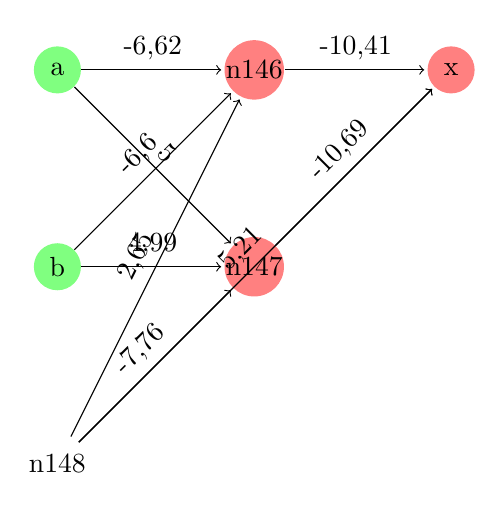
\begin{tikzpicture}[shorten >=1pt,->,draw=black!,node distance=2.5cm]
\tikzstyle{neuron}=[circle,fill=black!25,minimum size=17pt,inner sep=0pt]
\tikzstyle{constant}=[neuron, fill=white!50];
\tikzstyle{sigmoid}=[neuron, fill=red!50];
\tikzstyle{identity}=[neuron, fill=green!50];
\node [identity] (a) {a};
\node [identity,below of=a] (b) {b};
\node [constant,below of=b] (n148) {n148};
\node [sigmoid,right of=a] (n146) {n146};
\node [sigmoid,below of=n146] (n147) {n147};
\node [sigmoid,right of=n146] (x) {x};
\path[every node/.style={sloped,anchor=south,auto=false}]
(n146) edge node {-10,41} (x)
(n147) edge node {-10,69} (x)
(n148) edge node {-7,76} (n147)
(n148) edge node {2,65} (n146)
(n148) edge node {5,21} (x)
(a) edge node {5} (n147)
(a) edge node {-6,62} (n146)
(b) edge node {-6,6} (n146)
(b) edge node {4,99} (n147)
;\end{tikzpicture}
\end{document}